% Created by tikzDevice version 0.12.6 on 2026-02-05 18:38:49
% !TEX encoding = UTF-8 Unicode
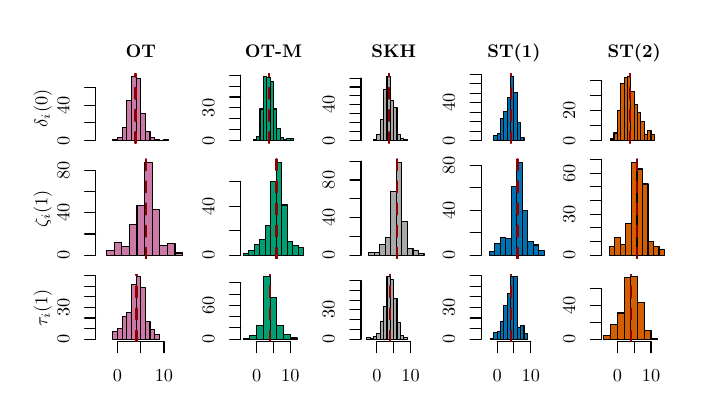
\begin{tikzpicture}[x=1pt,y=1pt]
\definecolor{fillColor}{RGB}{255,255,255}
\path[use as bounding box,fill=fillColor,fill opacity=0.00] (0,0) rectangle (234.15,130.09);
\begin{scope}
\path[clip] ( 24.55, 88.38) rectangle ( 57.18,113.45);
\definecolor{drawColor}{RGB}{0,0,0}
\definecolor{fillColor}{RGB}{204,121,167}

\path[draw=drawColor,line width= 0.4pt,line join=round,line cap=round,fill=fillColor] ( 30.80, 89.31) rectangle ( 32.47, 89.63);

\path[draw=drawColor,line width= 0.4pt,line join=round,line cap=round,fill=fillColor] ( 32.47, 89.31) rectangle ( 34.15, 90.26);

\path[draw=drawColor,line width= 0.4pt,line join=round,line cap=round,fill=fillColor] ( 34.15, 89.31) rectangle ( 35.83, 94.08);

\path[draw=drawColor,line width= 0.4pt,line join=round,line cap=round,fill=fillColor] ( 35.83, 89.31) rectangle ( 37.51,103.62);

\path[draw=drawColor,line width= 0.4pt,line join=round,line cap=round,fill=fillColor] ( 37.51, 89.31) rectangle ( 39.19,112.53);

\path[draw=drawColor,line width= 0.4pt,line join=round,line cap=round,fill=fillColor] ( 39.19, 89.31) rectangle ( 40.87,111.57);

\path[draw=drawColor,line width= 0.4pt,line join=round,line cap=round,fill=fillColor] ( 40.87, 89.31) rectangle ( 42.55, 99.17);

\path[draw=drawColor,line width= 0.4pt,line join=round,line cap=round,fill=fillColor] ( 42.55, 89.31) rectangle ( 44.22, 92.49);

\path[draw=drawColor,line width= 0.4pt,line join=round,line cap=round,fill=fillColor] ( 44.22, 89.31) rectangle ( 45.90, 90.26);

\path[draw=drawColor,line width= 0.4pt,line join=round,line cap=round,fill=fillColor] ( 45.90, 89.31) rectangle ( 47.58, 89.63);

\path[draw=drawColor,line width= 0.4pt,line join=round,line cap=round,fill=fillColor] ( 47.58, 89.31) rectangle ( 49.26, 89.31);

\path[draw=drawColor,line width= 0.4pt,line join=round,line cap=round,fill=fillColor] ( 49.26, 89.31) rectangle ( 50.94, 89.63);
\end{scope}
\begin{scope}
\path[clip] (  0.00,  0.00) rectangle (234.15,130.09);
\definecolor{drawColor}{RGB}{0,0,0}

\path[draw=drawColor,line width= 0.4pt,line join=round,line cap=round] ( 24.55, 89.31) -- ( 24.55,108.39);

\path[draw=drawColor,line width= 0.4pt,line join=round,line cap=round] ( 24.55, 89.31) -- ( 20.59, 89.31);

\path[draw=drawColor,line width= 0.4pt,line join=round,line cap=round] ( 24.55, 95.67) -- ( 20.59, 95.67);

\path[draw=drawColor,line width= 0.4pt,line join=round,line cap=round] ( 24.55,102.03) -- ( 20.59,102.03);

\path[draw=drawColor,line width= 0.4pt,line join=round,line cap=round] ( 24.55,108.39) -- ( 20.59,108.39);

\node[text=drawColor,rotate= 90.00,anchor=base,inner sep=0pt, outer sep=0pt, scale=  0.66] at ( 15.05, 89.31) {0};

\node[text=drawColor,rotate= 90.00,anchor=base,inner sep=0pt, outer sep=0pt, scale=  0.66] at ( 15.05,102.03) {40};
\end{scope}
\begin{scope}
\path[clip] (  0.00, 83.63) rectangle ( 60.35,130.09);
\definecolor{drawColor}{RGB}{0,0,0}

\node[text=drawColor,anchor=base,inner sep=0pt, outer sep=0pt, scale=  0.66] at ( 40.87,119.49) {\bfseries OT};

\node[text=drawColor,rotate= 90.00,anchor=base,inner sep=0pt, outer sep=0pt, scale=  0.66] at (  7.13,100.92) {$\delta_i(0)$};
\end{scope}
\begin{scope}
\path[clip] ( 24.55, 88.38) rectangle ( 57.18,113.45);
\definecolor{drawColor}{RGB}{139,0,0}

\path[draw=drawColor,line width= 0.8pt,dash pattern=on 4pt off 4pt ,line join=round,line cap=round] ( 38.99, 88.38) -- ( 38.99,113.45);
\end{scope}
\begin{scope}
\path[clip] ( 24.55, 46.57) rectangle ( 57.18, 82.83);
\definecolor{drawColor}{RGB}{0,0,0}
\definecolor{fillColor}{RGB}{204,121,167}

\path[draw=drawColor,line width= 0.4pt,line join=round,line cap=round,fill=fillColor] ( 28.51, 47.91) rectangle ( 31.25, 49.44);

\path[draw=drawColor,line width= 0.4pt,line join=round,line cap=round,fill=fillColor] ( 31.25, 47.91) rectangle ( 34.00, 52.49);

\path[draw=drawColor,line width= 0.4pt,line join=round,line cap=round,fill=fillColor] ( 34.00, 47.91) rectangle ( 36.75, 50.96);

\path[draw=drawColor,line width= 0.4pt,line join=round,line cap=round,fill=fillColor] ( 36.75, 47.91) rectangle ( 39.49, 58.98);

\path[draw=drawColor,line width= 0.4pt,line join=round,line cap=round,fill=fillColor] ( 39.49, 47.91) rectangle ( 42.24, 65.84);

\path[draw=drawColor,line width= 0.4pt,line join=round,line cap=round,fill=fillColor] ( 42.24, 47.91) rectangle ( 44.99, 81.49);

\path[draw=drawColor,line width= 0.4pt,line join=round,line cap=round,fill=fillColor] ( 44.99, 47.91) rectangle ( 47.73, 64.32);

\path[draw=drawColor,line width= 0.4pt,line join=round,line cap=round,fill=fillColor] ( 47.73, 47.91) rectangle ( 50.48, 51.34);

\path[draw=drawColor,line width= 0.4pt,line join=round,line cap=round,fill=fillColor] ( 50.48, 47.91) rectangle ( 53.23, 52.11);

\path[draw=drawColor,line width= 0.4pt,line join=round,line cap=round,fill=fillColor] ( 53.23, 47.91) rectangle ( 55.97, 48.67);
\end{scope}
\begin{scope}
\path[clip] (  0.00,  0.00) rectangle (234.15,130.09);
\definecolor{drawColor}{RGB}{0,0,0}

\path[draw=drawColor,line width= 0.4pt,line join=round,line cap=round] ( 24.55, 47.91) -- ( 24.55, 78.44);

\path[draw=drawColor,line width= 0.4pt,line join=round,line cap=round] ( 24.55, 47.91) -- ( 20.59, 47.91);

\path[draw=drawColor,line width= 0.4pt,line join=round,line cap=round] ( 24.55, 55.54) -- ( 20.59, 55.54);

\path[draw=drawColor,line width= 0.4pt,line join=round,line cap=round] ( 24.55, 63.17) -- ( 20.59, 63.17);

\path[draw=drawColor,line width= 0.4pt,line join=round,line cap=round] ( 24.55, 70.81) -- ( 20.59, 70.81);

\path[draw=drawColor,line width= 0.4pt,line join=round,line cap=round] ( 24.55, 78.44) -- ( 20.59, 78.44);

\node[text=drawColor,rotate= 90.00,anchor=base,inner sep=0pt, outer sep=0pt, scale=  0.66] at ( 15.05, 47.91) {0};

\node[text=drawColor,rotate= 90.00,anchor=base,inner sep=0pt, outer sep=0pt, scale=  0.66] at ( 15.05, 63.17) {40};

\node[text=drawColor,rotate= 90.00,anchor=base,inner sep=0pt, outer sep=0pt, scale=  0.66] at ( 15.05, 78.44) {80};
\end{scope}
\begin{scope}
\path[clip] (  0.00, 41.81) rectangle ( 60.35, 83.63);
\definecolor{drawColor}{RGB}{0,0,0}

\node[text=drawColor,rotate= 90.00,anchor=base,inner sep=0pt, outer sep=0pt, scale=  0.66] at (  7.13, 64.70) {$\zeta_i(1)$};
\end{scope}
\begin{scope}
\path[clip] ( 24.55, 46.57) rectangle ( 57.18, 82.83);
\definecolor{drawColor}{RGB}{139,0,0}

\path[draw=drawColor,line width= 0.8pt,dash pattern=on 4pt off 4pt ,line join=round,line cap=round] ( 42.66, 46.57) -- ( 42.66, 82.83);
\end{scope}
\begin{scope}
\path[clip] ( 24.55, 16.63) rectangle ( 57.18, 41.02);
\definecolor{drawColor}{RGB}{0,0,0}
\definecolor{fillColor}{RGB}{204,121,167}

\path[draw=drawColor,line width= 0.4pt,line join=round,line cap=round,fill=fillColor] ( 30.80, 17.54) rectangle ( 32.47, 20.21);

\path[draw=drawColor,line width= 0.4pt,line join=round,line cap=round,fill=fillColor] ( 32.47, 17.54) rectangle ( 34.15, 21.36);

\path[draw=drawColor,line width= 0.4pt,line join=round,line cap=round,fill=fillColor] ( 34.15, 17.54) rectangle ( 35.83, 25.57);

\path[draw=drawColor,line width= 0.4pt,line join=round,line cap=round,fill=fillColor] ( 35.83, 17.54) rectangle ( 37.51, 27.10);

\path[draw=drawColor,line width= 0.4pt,line join=round,line cap=round,fill=fillColor] ( 37.51, 17.54) rectangle ( 39.19, 37.44);

\path[draw=drawColor,line width= 0.4pt,line join=round,line cap=round,fill=fillColor] ( 39.19, 17.54) rectangle ( 40.87, 40.12);

\path[draw=drawColor,line width= 0.4pt,line join=round,line cap=round,fill=fillColor] ( 40.87, 17.54) rectangle ( 42.55, 36.29);

\path[draw=drawColor,line width= 0.4pt,line join=round,line cap=round,fill=fillColor] ( 42.55, 17.54) rectangle ( 44.22, 24.04);

\path[draw=drawColor,line width= 0.4pt,line join=round,line cap=round,fill=fillColor] ( 44.22, 17.54) rectangle ( 45.90, 20.98);

\path[draw=drawColor,line width= 0.4pt,line join=round,line cap=round,fill=fillColor] ( 45.90, 17.54) rectangle ( 47.58, 19.07);
\end{scope}
\begin{scope}
\path[clip] (  0.00,  0.00) rectangle (234.15,130.09);
\definecolor{drawColor}{RGB}{0,0,0}

\path[draw=drawColor,line width= 0.4pt,line join=round,line cap=round] ( 32.47, 16.63) -- ( 49.26, 16.63);

\path[draw=drawColor,line width= 0.4pt,line join=round,line cap=round] ( 32.47, 16.63) -- ( 32.47, 12.67);

\path[draw=drawColor,line width= 0.4pt,line join=round,line cap=round] ( 40.87, 16.63) -- ( 40.87, 12.67);

\path[draw=drawColor,line width= 0.4pt,line join=round,line cap=round] ( 49.26, 16.63) -- ( 49.26, 12.67);

\node[text=drawColor,anchor=base,inner sep=0pt, outer sep=0pt, scale=  0.66] at ( 32.47,  2.38) {0};

\node[text=drawColor,anchor=base,inner sep=0pt, outer sep=0pt, scale=  0.66] at ( 49.26,  2.38) {10};

\path[draw=drawColor,line width= 0.4pt,line join=round,line cap=round] ( 24.55, 17.54) -- ( 24.55, 40.50);

\path[draw=drawColor,line width= 0.4pt,line join=round,line cap=round] ( 24.55, 17.54) -- ( 20.59, 17.54);

\path[draw=drawColor,line width= 0.4pt,line join=round,line cap=round] ( 24.55, 21.36) -- ( 20.59, 21.36);

\path[draw=drawColor,line width= 0.4pt,line join=round,line cap=round] ( 24.55, 25.19) -- ( 20.59, 25.19);

\path[draw=drawColor,line width= 0.4pt,line join=round,line cap=round] ( 24.55, 29.02) -- ( 20.59, 29.02);

\path[draw=drawColor,line width= 0.4pt,line join=round,line cap=round] ( 24.55, 32.85) -- ( 20.59, 32.85);

\path[draw=drawColor,line width= 0.4pt,line join=round,line cap=round] ( 24.55, 36.67) -- ( 20.59, 36.67);

\path[draw=drawColor,line width= 0.4pt,line join=round,line cap=round] ( 24.55, 40.50) -- ( 20.59, 40.50);

\node[text=drawColor,rotate= 90.00,anchor=base,inner sep=0pt, outer sep=0pt, scale=  0.66] at ( 15.05, 17.54) {0};

\node[text=drawColor,rotate= 90.00,anchor=base,inner sep=0pt, outer sep=0pt, scale=  0.66] at ( 15.05, 29.02) {30};
\end{scope}
\begin{scope}
\path[clip] (  0.00,  0.00) rectangle ( 60.35, 41.81);
\definecolor{drawColor}{RGB}{0,0,0}

\node[text=drawColor,rotate= 90.00,anchor=base,inner sep=0pt, outer sep=0pt, scale=  0.66] at (  7.13, 28.83) {$\tau_i(1)$};
\end{scope}
\begin{scope}
\path[clip] ( 24.55, 16.63) rectangle ( 57.18, 41.02);
\definecolor{drawColor}{RGB}{139,0,0}

\path[draw=drawColor,line width= 0.8pt,dash pattern=on 4pt off 4pt ,line join=round,line cap=round] ( 39.35, 16.63) -- ( 39.35, 41.02);
\end{scope}
\begin{scope}
\path[clip] ( 76.98, 88.38) rectangle (100.63,113.45);
\definecolor{drawColor}{RGB}{0,0,0}
\definecolor{fillColor}{RGB}{0,158,115}

\path[draw=drawColor,line width= 0.4pt,line join=round,line cap=round,fill=fillColor] ( 81.51, 89.31) rectangle ( 82.72, 89.70);

\path[draw=drawColor,line width= 0.4pt,line join=round,line cap=round,fill=fillColor] ( 82.72, 89.31) rectangle ( 83.94, 90.88);

\path[draw=drawColor,line width= 0.4pt,line join=round,line cap=round,fill=fillColor] ( 83.94, 89.31) rectangle ( 85.16,100.72);

\path[draw=drawColor,line width= 0.4pt,line join=round,line cap=round,fill=fillColor] ( 85.16, 89.31) rectangle ( 86.37,112.53);

\path[draw=drawColor,line width= 0.4pt,line join=round,line cap=round,fill=fillColor] ( 86.37, 89.31) rectangle ( 87.59,112.13);

\path[draw=drawColor,line width= 0.4pt,line join=round,line cap=round,fill=fillColor] ( 87.59, 89.31) rectangle ( 88.81,110.56);

\path[draw=drawColor,line width= 0.4pt,line join=round,line cap=round,fill=fillColor] ( 88.81, 89.31) rectangle ( 90.02,100.72);

\path[draw=drawColor,line width= 0.4pt,line join=round,line cap=round,fill=fillColor] ( 90.02, 89.31) rectangle ( 91.24, 93.64);

\path[draw=drawColor,line width= 0.4pt,line join=round,line cap=round,fill=fillColor] ( 91.24, 89.31) rectangle ( 92.46, 90.49);

\path[draw=drawColor,line width= 0.4pt,line join=round,line cap=round,fill=fillColor] ( 92.46, 89.31) rectangle ( 93.67, 89.70);

\path[draw=drawColor,line width= 0.4pt,line join=round,line cap=round,fill=fillColor] ( 93.67, 89.31) rectangle ( 94.89, 90.09);

\path[draw=drawColor,line width= 0.4pt,line join=round,line cap=round,fill=fillColor] ( 94.89, 89.31) rectangle ( 96.11, 90.09);
\end{scope}
\begin{scope}
\path[clip] (  0.00,  0.00) rectangle (234.15,130.09);
\definecolor{drawColor}{RGB}{0,0,0}

\path[draw=drawColor,line width= 0.4pt,line join=round,line cap=round] ( 76.98, 89.31) -- ( 76.98,112.92);

\path[draw=drawColor,line width= 0.4pt,line join=round,line cap=round] ( 76.98, 89.31) -- ( 73.02, 89.31);

\path[draw=drawColor,line width= 0.4pt,line join=round,line cap=round] ( 76.98, 93.24) -- ( 73.02, 93.24);

\path[draw=drawColor,line width= 0.4pt,line join=round,line cap=round] ( 76.98, 97.18) -- ( 73.02, 97.18);

\path[draw=drawColor,line width= 0.4pt,line join=round,line cap=round] ( 76.98,101.11) -- ( 73.02,101.11);

\path[draw=drawColor,line width= 0.4pt,line join=round,line cap=round] ( 76.98,105.05) -- ( 73.02,105.05);

\path[draw=drawColor,line width= 0.4pt,line join=round,line cap=round] ( 76.98,108.98) -- ( 73.02,108.98);

\path[draw=drawColor,line width= 0.4pt,line join=round,line cap=round] ( 76.98,112.92) -- ( 73.02,112.92);

\node[text=drawColor,rotate= 90.00,anchor=base,inner sep=0pt, outer sep=0pt, scale=  0.66] at ( 67.48, 89.31) {0};

\node[text=drawColor,rotate= 90.00,anchor=base,inner sep=0pt, outer sep=0pt, scale=  0.66] at ( 67.48,101.11) {30};
\end{scope}
\begin{scope}
\path[clip] ( 60.35, 83.63) rectangle (103.80,130.09);
\definecolor{drawColor}{RGB}{0,0,0}

\node[text=drawColor,anchor=base,inner sep=0pt, outer sep=0pt, scale=  0.66] at ( 88.81,119.49) {\bfseries OT-M};
\end{scope}
\begin{scope}
\path[clip] ( 76.98, 88.38) rectangle (100.63,113.45);
\definecolor{drawColor}{RGB}{139,0,0}

\path[draw=drawColor,line width= 0.8pt,dash pattern=on 4pt off 4pt ,line join=round,line cap=round] ( 87.25, 88.38) -- ( 87.25,113.45);
\end{scope}
\begin{scope}
\path[clip] ( 76.98, 46.57) rectangle (100.63, 82.83);
\definecolor{drawColor}{RGB}{0,0,0}
\definecolor{fillColor}{RGB}{0,158,115}

\path[draw=drawColor,line width= 0.4pt,line join=round,line cap=round,fill=fillColor] ( 77.86, 47.91) rectangle ( 79.85, 48.35);

\path[draw=drawColor,line width= 0.4pt,line join=round,line cap=round,fill=fillColor] ( 79.85, 47.91) rectangle ( 81.84, 49.68);

\path[draw=drawColor,line width= 0.4pt,line join=round,line cap=round,fill=fillColor] ( 81.84, 47.91) rectangle ( 83.83, 51.89);

\path[draw=drawColor,line width= 0.4pt,line join=round,line cap=round,fill=fillColor] ( 83.83, 47.91) rectangle ( 85.82, 53.65);

\path[draw=drawColor,line width= 0.4pt,line join=round,line cap=round,fill=fillColor] ( 85.82, 47.91) rectangle ( 87.81, 58.51);

\path[draw=drawColor,line width= 0.4pt,line join=round,line cap=round,fill=fillColor] ( 87.81, 47.91) rectangle ( 89.80, 74.42);

\path[draw=drawColor,line width= 0.4pt,line join=round,line cap=round,fill=fillColor] ( 89.80, 47.91) rectangle ( 91.79, 81.49);

\path[draw=drawColor,line width= 0.4pt,line join=round,line cap=round,fill=fillColor] ( 91.79, 47.91) rectangle ( 93.78, 66.03);

\path[draw=drawColor,line width= 0.4pt,line join=round,line cap=round,fill=fillColor] ( 93.78, 47.91) rectangle ( 95.77, 52.77);

\path[draw=drawColor,line width= 0.4pt,line join=round,line cap=round,fill=fillColor] ( 95.77, 47.91) rectangle ( 97.77, 51.44);

\path[draw=drawColor,line width= 0.4pt,line join=round,line cap=round,fill=fillColor] ( 97.77, 47.91) rectangle ( 99.76, 50.56);
\end{scope}
\begin{scope}
\path[clip] (  0.00,  0.00) rectangle (234.15,130.09);
\definecolor{drawColor}{RGB}{0,0,0}

\path[draw=drawColor,line width= 0.4pt,line join=round,line cap=round] ( 76.98, 47.91) -- ( 76.98, 74.42);

\path[draw=drawColor,line width= 0.4pt,line join=round,line cap=round] ( 76.98, 47.91) -- ( 73.02, 47.91);

\path[draw=drawColor,line width= 0.4pt,line join=round,line cap=round] ( 76.98, 56.75) -- ( 73.02, 56.75);

\path[draw=drawColor,line width= 0.4pt,line join=round,line cap=round] ( 76.98, 65.58) -- ( 73.02, 65.58);

\path[draw=drawColor,line width= 0.4pt,line join=round,line cap=round] ( 76.98, 74.42) -- ( 73.02, 74.42);

\node[text=drawColor,rotate= 90.00,anchor=base,inner sep=0pt, outer sep=0pt, scale=  0.66] at ( 67.48, 47.91) {0};

\node[text=drawColor,rotate= 90.00,anchor=base,inner sep=0pt, outer sep=0pt, scale=  0.66] at ( 67.48, 65.58) {40};
\end{scope}
\begin{scope}
\path[clip] ( 76.98, 46.57) rectangle (100.63, 82.83);
\definecolor{drawColor}{RGB}{139,0,0}

\path[draw=drawColor,line width= 0.8pt,dash pattern=on 4pt off 4pt ,line join=round,line cap=round] ( 89.95, 46.57) -- ( 89.95, 82.83);
\end{scope}
\begin{scope}
\path[clip] ( 76.98, 16.63) rectangle (100.63, 41.02);
\definecolor{drawColor}{RGB}{0,0,0}
\definecolor{fillColor}{RGB}{0,158,115}

\path[draw=drawColor,line width= 0.4pt,line join=round,line cap=round,fill=fillColor] ( 77.86, 17.54) rectangle ( 80.29, 17.74);

\path[draw=drawColor,line width= 0.4pt,line join=round,line cap=round,fill=fillColor] ( 80.29, 17.54) rectangle ( 82.72, 18.76);

\path[draw=drawColor,line width= 0.4pt,line join=round,line cap=round,fill=fillColor] ( 82.72, 17.54) rectangle ( 85.16, 22.62);

\path[draw=drawColor,line width= 0.4pt,line join=round,line cap=round,fill=fillColor] ( 85.16, 17.54) rectangle ( 87.59, 40.12);

\path[draw=drawColor,line width= 0.4pt,line join=round,line cap=round,fill=fillColor] ( 87.59, 17.54) rectangle ( 90.02, 32.59);

\path[draw=drawColor,line width= 0.4pt,line join=round,line cap=round,fill=fillColor] ( 90.02, 17.54) rectangle ( 92.46, 22.62);

\path[draw=drawColor,line width= 0.4pt,line join=round,line cap=round,fill=fillColor] ( 92.46, 17.54) rectangle ( 94.89, 19.37);

\path[draw=drawColor,line width= 0.4pt,line join=round,line cap=round,fill=fillColor] ( 94.89, 17.54) rectangle ( 97.32, 17.94);
\end{scope}
\begin{scope}
\path[clip] (  0.00,  0.00) rectangle (234.15,130.09);
\definecolor{drawColor}{RGB}{0,0,0}

\path[draw=drawColor,line width= 0.4pt,line join=round,line cap=round] ( 82.72, 16.63) -- ( 94.89, 16.63);

\path[draw=drawColor,line width= 0.4pt,line join=round,line cap=round] ( 82.72, 16.63) -- ( 82.72, 12.67);

\path[draw=drawColor,line width= 0.4pt,line join=round,line cap=round] ( 88.81, 16.63) -- ( 88.81, 12.67);

\path[draw=drawColor,line width= 0.4pt,line join=round,line cap=round] ( 94.89, 16.63) -- ( 94.89, 12.67);

\node[text=drawColor,anchor=base,inner sep=0pt, outer sep=0pt, scale=  0.66] at ( 82.72,  2.38) {0};

\node[text=drawColor,anchor=base,inner sep=0pt, outer sep=0pt, scale=  0.66] at ( 94.89,  2.38) {10};

\path[draw=drawColor,line width= 0.4pt,line join=round,line cap=round] ( 76.98, 17.54) -- ( 76.98, 37.88);

\path[draw=drawColor,line width= 0.4pt,line join=round,line cap=round] ( 76.98, 17.54) -- ( 73.02, 17.54);

\path[draw=drawColor,line width= 0.4pt,line join=round,line cap=round] ( 76.98, 21.60) -- ( 73.02, 21.60);

\path[draw=drawColor,line width= 0.4pt,line join=round,line cap=round] ( 76.98, 25.67) -- ( 73.02, 25.67);

\path[draw=drawColor,line width= 0.4pt,line join=round,line cap=round] ( 76.98, 29.74) -- ( 73.02, 29.74);

\path[draw=drawColor,line width= 0.4pt,line join=round,line cap=round] ( 76.98, 33.81) -- ( 73.02, 33.81);

\path[draw=drawColor,line width= 0.4pt,line join=round,line cap=round] ( 76.98, 37.88) -- ( 73.02, 37.88);

\node[text=drawColor,rotate= 90.00,anchor=base,inner sep=0pt, outer sep=0pt, scale=  0.66] at ( 67.48, 17.54) {0};

\node[text=drawColor,rotate= 90.00,anchor=base,inner sep=0pt, outer sep=0pt, scale=  0.66] at ( 67.48, 29.74) {60};
\end{scope}
\begin{scope}
\path[clip] ( 76.98, 16.63) rectangle (100.63, 41.02);
\definecolor{drawColor}{RGB}{139,0,0}

\path[draw=drawColor,line width= 0.8pt,dash pattern=on 4pt off 4pt ,line join=round,line cap=round] ( 87.51, 16.63) -- ( 87.51, 41.02);
\end{scope}
\begin{scope}
\path[clip] (120.43, 88.38) rectangle (144.08,113.45);
\definecolor{drawColor}{RGB}{0,0,0}
\definecolor{fillColor}{RGB}{169,169,169}

\path[draw=drawColor,line width= 0.4pt,line join=round,line cap=round,fill=fillColor] (124.96, 89.31) rectangle (126.18, 89.63);

\path[draw=drawColor,line width= 0.4pt,line join=round,line cap=round,fill=fillColor] (126.18, 89.31) rectangle (127.39, 91.56);

\path[draw=drawColor,line width= 0.4pt,line join=round,line cap=round,fill=fillColor] (127.39, 89.31) rectangle (128.61, 97.05);

\path[draw=drawColor,line width= 0.4pt,line join=round,line cap=round,fill=fillColor] (128.61, 89.31) rectangle (129.83,107.69);

\path[draw=drawColor,line width= 0.4pt,line join=round,line cap=round,fill=fillColor] (129.83, 89.31) rectangle (131.04,112.53);

\path[draw=drawColor,line width= 0.4pt,line join=round,line cap=round,fill=fillColor] (131.04, 89.31) rectangle (132.26,103.82);

\path[draw=drawColor,line width= 0.4pt,line join=round,line cap=round,fill=fillColor] (132.26, 89.31) rectangle (133.47,101.24);

\path[draw=drawColor,line width= 0.4pt,line join=round,line cap=round,fill=fillColor] (133.47, 89.31) rectangle (134.69, 91.56);

\path[draw=drawColor,line width= 0.4pt,line join=round,line cap=round,fill=fillColor] (134.69, 89.31) rectangle (135.91, 89.95);

\path[draw=drawColor,line width= 0.4pt,line join=round,line cap=round,fill=fillColor] (135.91, 89.31) rectangle (137.12, 89.63);
\end{scope}
\begin{scope}
\path[clip] (  0.00,  0.00) rectangle (234.15,130.09);
\definecolor{drawColor}{RGB}{0,0,0}

\path[draw=drawColor,line width= 0.4pt,line join=round,line cap=round] (120.43, 89.31) -- (120.43,111.88);

\path[draw=drawColor,line width= 0.4pt,line join=round,line cap=round] (120.43, 89.31) -- (116.47, 89.31);

\path[draw=drawColor,line width= 0.4pt,line join=round,line cap=round] (120.43, 92.53) -- (116.47, 92.53);

\path[draw=drawColor,line width= 0.4pt,line join=round,line cap=round] (120.43, 95.76) -- (116.47, 95.76);

\path[draw=drawColor,line width= 0.4pt,line join=round,line cap=round] (120.43, 98.98) -- (116.47, 98.98);

\path[draw=drawColor,line width= 0.4pt,line join=round,line cap=round] (120.43,102.21) -- (116.47,102.21);

\path[draw=drawColor,line width= 0.4pt,line join=round,line cap=round] (120.43,105.43) -- (116.47,105.43);

\path[draw=drawColor,line width= 0.4pt,line join=round,line cap=round] (120.43,108.66) -- (116.47,108.66);

\path[draw=drawColor,line width= 0.4pt,line join=round,line cap=round] (120.43,111.88) -- (116.47,111.88);

\node[text=drawColor,rotate= 90.00,anchor=base,inner sep=0pt, outer sep=0pt, scale=  0.66] at (110.93, 89.31) {0};

\node[text=drawColor,rotate= 90.00,anchor=base,inner sep=0pt, outer sep=0pt, scale=  0.66] at (110.93,102.21) {40};
\end{scope}
\begin{scope}
\path[clip] (103.80, 83.63) rectangle (147.25,130.09);
\definecolor{drawColor}{RGB}{0,0,0}

\node[text=drawColor,anchor=base,inner sep=0pt, outer sep=0pt, scale=  0.66] at (132.26,119.49) {\bfseries SKH};
\end{scope}
\begin{scope}
\path[clip] (120.43, 88.38) rectangle (144.08,113.45);
\definecolor{drawColor}{RGB}{139,0,0}

\path[draw=drawColor,line width= 0.8pt,dash pattern=on 4pt off 4pt ,line join=round,line cap=round] (130.54, 88.38) -- (130.54,113.45);
\end{scope}
\begin{scope}
\path[clip] (120.43, 46.57) rectangle (144.08, 82.83);
\definecolor{drawColor}{RGB}{0,0,0}
\definecolor{fillColor}{RGB}{169,169,169}

\path[draw=drawColor,line width= 0.4pt,line join=round,line cap=round,fill=fillColor] (123.30, 47.91) rectangle (125.29, 48.93);

\path[draw=drawColor,line width= 0.4pt,line join=round,line cap=round,fill=fillColor] (125.29, 47.91) rectangle (127.28, 48.93);

\path[draw=drawColor,line width= 0.4pt,line join=round,line cap=round,fill=fillColor] (127.28, 47.91) rectangle (129.27, 51.64);

\path[draw=drawColor,line width= 0.4pt,line join=round,line cap=round,fill=fillColor] (129.27, 47.91) rectangle (131.26, 54.35);

\path[draw=drawColor,line width= 0.4pt,line join=round,line cap=round,fill=fillColor] (131.26, 47.91) rectangle (133.25, 70.98);

\path[draw=drawColor,line width= 0.4pt,line join=round,line cap=round,fill=fillColor] (133.25, 47.91) rectangle (135.24, 81.49);

\path[draw=drawColor,line width= 0.4pt,line join=round,line cap=round,fill=fillColor] (135.24, 47.91) rectangle (137.24, 60.12);

\path[draw=drawColor,line width= 0.4pt,line join=round,line cap=round,fill=fillColor] (137.24, 47.91) rectangle (139.23, 50.28);

\path[draw=drawColor,line width= 0.4pt,line join=round,line cap=round,fill=fillColor] (139.23, 47.91) rectangle (141.22, 49.60);

\path[draw=drawColor,line width= 0.4pt,line join=round,line cap=round,fill=fillColor] (141.22, 47.91) rectangle (143.21, 48.59);
\end{scope}
\begin{scope}
\path[clip] (  0.00,  0.00) rectangle (234.15,130.09);
\definecolor{drawColor}{RGB}{0,0,0}

\path[draw=drawColor,line width= 0.4pt,line join=round,line cap=round] (120.43, 47.91) -- (120.43, 81.83);

\path[draw=drawColor,line width= 0.4pt,line join=round,line cap=round] (120.43, 47.91) -- (116.47, 47.91);

\path[draw=drawColor,line width= 0.4pt,line join=round,line cap=round] (120.43, 54.69) -- (116.47, 54.69);

\path[draw=drawColor,line width= 0.4pt,line join=round,line cap=round] (120.43, 61.48) -- (116.47, 61.48);

\path[draw=drawColor,line width= 0.4pt,line join=round,line cap=round] (120.43, 68.26) -- (116.47, 68.26);

\path[draw=drawColor,line width= 0.4pt,line join=round,line cap=round] (120.43, 75.05) -- (116.47, 75.05);

\path[draw=drawColor,line width= 0.4pt,line join=round,line cap=round] (120.43, 81.83) -- (116.47, 81.83);

\node[text=drawColor,rotate= 90.00,anchor=base,inner sep=0pt, outer sep=0pt, scale=  0.66] at (110.93, 47.91) {0};

\node[text=drawColor,rotate= 90.00,anchor=base,inner sep=0pt, outer sep=0pt, scale=  0.66] at (110.93, 61.48) {40};

\node[text=drawColor,rotate= 90.00,anchor=base,inner sep=0pt, outer sep=0pt, scale=  0.66] at (110.93, 75.05) {80};
\end{scope}
\begin{scope}
\path[clip] (120.43, 46.57) rectangle (144.08, 82.83);
\definecolor{drawColor}{RGB}{139,0,0}

\path[draw=drawColor,line width= 0.8pt,dash pattern=on 4pt off 4pt ,line join=round,line cap=round] (133.50, 46.57) -- (133.50, 82.83);
\end{scope}
\begin{scope}
\path[clip] (120.43, 16.63) rectangle (144.08, 41.02);
\definecolor{drawColor}{RGB}{0,0,0}
\definecolor{fillColor}{RGB}{169,169,169}

\path[draw=drawColor,line width= 0.4pt,line join=round,line cap=round,fill=fillColor] (122.53, 17.54) rectangle (123.74, 18.24);

\path[draw=drawColor,line width= 0.4pt,line join=round,line cap=round,fill=fillColor] (123.74, 17.54) rectangle (124.96, 17.89);

\path[draw=drawColor,line width= 0.4pt,line join=round,line cap=round,fill=fillColor] (124.96, 17.54) rectangle (126.18, 18.59);

\path[draw=drawColor,line width= 0.4pt,line join=round,line cap=round,fill=fillColor] (126.18, 17.54) rectangle (127.39, 19.65);

\path[draw=drawColor,line width= 0.4pt,line join=round,line cap=round,fill=fillColor] (127.39, 17.54) rectangle (128.61, 23.89);

\path[draw=drawColor,line width= 0.4pt,line join=round,line cap=round,fill=fillColor] (128.61, 17.54) rectangle (129.83, 29.18);

\path[draw=drawColor,line width= 0.4pt,line join=round,line cap=round,fill=fillColor] (129.83, 17.54) rectangle (131.04, 40.12);

\path[draw=drawColor,line width= 0.4pt,line join=round,line cap=round,fill=fillColor] (131.04, 17.54) rectangle (132.26, 39.06);

\path[draw=drawColor,line width= 0.4pt,line join=round,line cap=round,fill=fillColor] (132.26, 17.54) rectangle (133.47, 32.36);

\path[draw=drawColor,line width= 0.4pt,line join=round,line cap=round,fill=fillColor] (133.47, 17.54) rectangle (134.69, 23.53);

\path[draw=drawColor,line width= 0.4pt,line join=round,line cap=round,fill=fillColor] (134.69, 17.54) rectangle (135.91, 18.95);

\path[draw=drawColor,line width= 0.4pt,line join=round,line cap=round,fill=fillColor] (135.91, 17.54) rectangle (137.12, 18.24);
\end{scope}
\begin{scope}
\path[clip] (  0.00,  0.00) rectangle (234.15,130.09);
\definecolor{drawColor}{RGB}{0,0,0}

\path[draw=drawColor,line width= 0.4pt,line join=round,line cap=round] (126.18, 16.63) -- (138.34, 16.63);

\path[draw=drawColor,line width= 0.4pt,line join=round,line cap=round] (126.18, 16.63) -- (126.18, 12.67);

\path[draw=drawColor,line width= 0.4pt,line join=round,line cap=round] (132.26, 16.63) -- (132.26, 12.67);

\path[draw=drawColor,line width= 0.4pt,line join=round,line cap=round] (138.34, 16.63) -- (138.34, 12.67);

\node[text=drawColor,anchor=base,inner sep=0pt, outer sep=0pt, scale=  0.66] at (126.18,  2.38) {0};

\node[text=drawColor,anchor=base,inner sep=0pt, outer sep=0pt, scale=  0.66] at (138.34,  2.38) {10};

\path[draw=drawColor,line width= 0.4pt,line join=round,line cap=round] (120.43, 17.54) -- (120.43, 38.71);

\path[draw=drawColor,line width= 0.4pt,line join=round,line cap=round] (120.43, 17.54) -- (116.47, 17.54);

\path[draw=drawColor,line width= 0.4pt,line join=round,line cap=round] (120.43, 21.06) -- (116.47, 21.06);

\path[draw=drawColor,line width= 0.4pt,line join=round,line cap=round] (120.43, 24.59) -- (116.47, 24.59);

\path[draw=drawColor,line width= 0.4pt,line join=round,line cap=round] (120.43, 28.12) -- (116.47, 28.12);

\path[draw=drawColor,line width= 0.4pt,line join=round,line cap=round] (120.43, 31.65) -- (116.47, 31.65);

\path[draw=drawColor,line width= 0.4pt,line join=round,line cap=round] (120.43, 35.18) -- (116.47, 35.18);

\path[draw=drawColor,line width= 0.4pt,line join=round,line cap=round] (120.43, 38.71) -- (116.47, 38.71);

\node[text=drawColor,rotate= 90.00,anchor=base,inner sep=0pt, outer sep=0pt, scale=  0.66] at (110.93, 17.54) {0};

\node[text=drawColor,rotate= 90.00,anchor=base,inner sep=0pt, outer sep=0pt, scale=  0.66] at (110.93, 28.12) {30};
\end{scope}
\begin{scope}
\path[clip] (120.43, 16.63) rectangle (144.08, 41.02);
\definecolor{drawColor}{RGB}{139,0,0}

\path[draw=drawColor,line width= 0.8pt,dash pattern=on 4pt off 4pt ,line join=round,line cap=round] (130.94, 16.63) -- (130.94, 41.02);
\end{scope}
\begin{scope}
\path[clip] (163.88, 88.38) rectangle (187.54,113.45);
\definecolor{drawColor}{RGB}{0,0,0}
\definecolor{fillColor}{RGB}{0,114,178}

\path[draw=drawColor,line width= 0.4pt,line join=round,line cap=round,fill=fillColor] (168.41, 89.31) rectangle (169.63, 91.01);

\path[draw=drawColor,line width= 0.4pt,line join=round,line cap=round,fill=fillColor] (169.63, 89.31) rectangle (170.84, 91.70);

\path[draw=drawColor,line width= 0.4pt,line join=round,line cap=round,fill=fillColor] (170.84, 89.31) rectangle (172.06, 97.16);

\path[draw=drawColor,line width= 0.4pt,line join=round,line cap=round,fill=fillColor] (172.06, 89.31) rectangle (173.28, 99.89);

\path[draw=drawColor,line width= 0.4pt,line join=round,line cap=round,fill=fillColor] (173.28, 89.31) rectangle (174.49,105.01);

\path[draw=drawColor,line width= 0.4pt,line join=round,line cap=round,fill=fillColor] (174.49, 89.31) rectangle (175.71,112.53);

\path[draw=drawColor,line width= 0.4pt,line join=round,line cap=round,fill=fillColor] (175.71, 89.31) rectangle (176.93,106.72);

\path[draw=drawColor,line width= 0.4pt,line join=round,line cap=round,fill=fillColor] (176.93, 89.31) rectangle (178.14, 95.79);

\path[draw=drawColor,line width= 0.4pt,line join=round,line cap=round,fill=fillColor] (178.14, 89.31) rectangle (179.36, 90.33);
\end{scope}
\begin{scope}
\path[clip] (  0.00,  0.00) rectangle (234.15,130.09);
\definecolor{drawColor}{RGB}{0,0,0}

\path[draw=drawColor,line width= 0.4pt,line join=round,line cap=round] (163.88, 89.31) -- (163.88,113.21);

\path[draw=drawColor,line width= 0.4pt,line join=round,line cap=round] (163.88, 89.31) -- (159.92, 89.31);

\path[draw=drawColor,line width= 0.4pt,line join=round,line cap=round] (163.88, 92.72) -- (159.92, 92.72);

\path[draw=drawColor,line width= 0.4pt,line join=round,line cap=round] (163.88, 96.14) -- (159.92, 96.14);

\path[draw=drawColor,line width= 0.4pt,line join=round,line cap=round] (163.88, 99.55) -- (159.92, 99.55);

\path[draw=drawColor,line width= 0.4pt,line join=round,line cap=round] (163.88,102.96) -- (159.92,102.96);

\path[draw=drawColor,line width= 0.4pt,line join=round,line cap=round] (163.88,106.38) -- (159.92,106.38);

\path[draw=drawColor,line width= 0.4pt,line join=round,line cap=round] (163.88,109.79) -- (159.92,109.79);

\path[draw=drawColor,line width= 0.4pt,line join=round,line cap=round] (163.88,113.21) -- (159.92,113.21);

\node[text=drawColor,rotate= 90.00,anchor=base,inner sep=0pt, outer sep=0pt, scale=  0.66] at (154.38, 89.31) {0};

\node[text=drawColor,rotate= 90.00,anchor=base,inner sep=0pt, outer sep=0pt, scale=  0.66] at (154.38,102.96) {40};
\end{scope}
\begin{scope}
\path[clip] (147.25, 83.63) rectangle (190.70,130.09);
\definecolor{drawColor}{RGB}{0,0,0}

\node[text=drawColor,anchor=base,inner sep=0pt, outer sep=0pt, scale=  0.66] at (175.71,119.49) {\bfseries ST(1)};
\end{scope}
\begin{scope}
\path[clip] (163.88, 88.38) rectangle (187.54,113.45);
\definecolor{drawColor}{RGB}{139,0,0}

\path[draw=drawColor,line width= 0.8pt,dash pattern=on 4pt off 4pt ,line join=round,line cap=round] (174.53, 88.38) -- (174.53,113.45);
\end{scope}
\begin{scope}
\path[clip] (163.88, 46.57) rectangle (187.54, 82.83);
\definecolor{drawColor}{RGB}{0,0,0}
\definecolor{fillColor}{RGB}{0,114,178}

\path[draw=drawColor,line width= 0.4pt,line join=round,line cap=round,fill=fillColor] (166.75, 47.91) rectangle (168.74, 49.12);

\path[draw=drawColor,line width= 0.4pt,line join=round,line cap=round,fill=fillColor] (168.74, 47.91) rectangle (170.73, 51.95);

\path[draw=drawColor,line width= 0.4pt,line join=round,line cap=round,fill=fillColor] (170.73, 47.91) rectangle (172.72, 54.38);

\path[draw=drawColor,line width= 0.4pt,line join=round,line cap=round,fill=fillColor] (172.72, 47.91) rectangle (174.71, 53.98);

\path[draw=drawColor,line width= 0.4pt,line join=round,line cap=round,fill=fillColor] (174.71, 47.91) rectangle (176.71, 72.59);

\path[draw=drawColor,line width= 0.4pt,line join=round,line cap=round,fill=fillColor] (176.71, 47.91) rectangle (178.70, 81.49);

\path[draw=drawColor,line width= 0.4pt,line join=round,line cap=round,fill=fillColor] (178.70, 47.91) rectangle (180.69, 64.09);

\path[draw=drawColor,line width= 0.4pt,line join=round,line cap=round,fill=fillColor] (180.69, 47.91) rectangle (182.68, 52.76);

\path[draw=drawColor,line width= 0.4pt,line join=round,line cap=round,fill=fillColor] (182.68, 47.91) rectangle (184.67, 51.55);

\path[draw=drawColor,line width= 0.4pt,line join=round,line cap=round,fill=fillColor] (184.67, 47.91) rectangle (186.66, 49.53);
\end{scope}
\begin{scope}
\path[clip] (  0.00,  0.00) rectangle (234.15,130.09);
\definecolor{drawColor}{RGB}{0,0,0}

\path[draw=drawColor,line width= 0.4pt,line join=round,line cap=round] (163.88, 47.91) -- (163.88, 80.28);

\path[draw=drawColor,line width= 0.4pt,line join=round,line cap=round] (163.88, 47.91) -- (159.92, 47.91);

\path[draw=drawColor,line width= 0.4pt,line join=round,line cap=round] (163.88, 56.00) -- (159.92, 56.00);

\path[draw=drawColor,line width= 0.4pt,line join=round,line cap=round] (163.88, 64.09) -- (159.92, 64.09);

\path[draw=drawColor,line width= 0.4pt,line join=round,line cap=round] (163.88, 72.19) -- (159.92, 72.19);

\path[draw=drawColor,line width= 0.4pt,line join=round,line cap=round] (163.88, 80.28) -- (159.92, 80.28);

\node[text=drawColor,rotate= 90.00,anchor=base,inner sep=0pt, outer sep=0pt, scale=  0.66] at (154.38, 47.91) {0};

\node[text=drawColor,rotate= 90.00,anchor=base,inner sep=0pt, outer sep=0pt, scale=  0.66] at (154.38, 64.09) {40};

\node[text=drawColor,rotate= 90.00,anchor=base,inner sep=0pt, outer sep=0pt, scale=  0.66] at (154.38, 80.28) {80};
\end{scope}
\begin{scope}
\path[clip] (163.88, 46.57) rectangle (187.54, 82.83);
\definecolor{drawColor}{RGB}{139,0,0}

\path[draw=drawColor,line width= 0.8pt,dash pattern=on 4pt off 4pt ,line join=round,line cap=round] (176.98, 46.57) -- (176.98, 82.83);
\end{scope}
\begin{scope}
\path[clip] (163.88, 16.63) rectangle (187.54, 41.02);
\definecolor{drawColor}{RGB}{0,0,0}
\definecolor{fillColor}{RGB}{0,114,178}

\path[draw=drawColor,line width= 0.4pt,line join=round,line cap=round,fill=fillColor] (167.19, 17.54) rectangle (168.41, 17.92);

\path[draw=drawColor,line width= 0.4pt,line join=round,line cap=round,fill=fillColor] (168.41, 17.54) rectangle (169.63, 19.83);

\path[draw=drawColor,line width= 0.4pt,line join=round,line cap=round,fill=fillColor] (169.63, 17.54) rectangle (170.84, 20.21);

\path[draw=drawColor,line width= 0.4pt,line join=round,line cap=round,fill=fillColor] (170.84, 17.54) rectangle (172.06, 24.04);

\path[draw=drawColor,line width= 0.4pt,line join=round,line cap=round,fill=fillColor] (172.06, 17.54) rectangle (173.28, 29.78);

\path[draw=drawColor,line width= 0.4pt,line join=round,line cap=round,fill=fillColor] (173.28, 17.54) rectangle (174.49, 33.99);

\path[draw=drawColor,line width= 0.4pt,line join=round,line cap=round,fill=fillColor] (174.49, 17.54) rectangle (175.71, 40.12);

\path[draw=drawColor,line width= 0.4pt,line join=round,line cap=round,fill=fillColor] (175.71, 17.54) rectangle (176.93, 40.12);

\path[draw=drawColor,line width= 0.4pt,line join=round,line cap=round,fill=fillColor] (176.93, 17.54) rectangle (178.14, 21.75);

\path[draw=drawColor,line width= 0.4pt,line join=round,line cap=round,fill=fillColor] (178.14, 17.54) rectangle (179.36, 22.51);

\path[draw=drawColor,line width= 0.4pt,line join=round,line cap=round,fill=fillColor] (179.36, 17.54) rectangle (180.58, 19.45);
\end{scope}
\begin{scope}
\path[clip] (  0.00,  0.00) rectangle (234.15,130.09);
\definecolor{drawColor}{RGB}{0,0,0}

\path[draw=drawColor,line width= 0.4pt,line join=round,line cap=round] (169.63, 16.63) -- (181.79, 16.63);

\path[draw=drawColor,line width= 0.4pt,line join=round,line cap=round] (169.63, 16.63) -- (169.63, 12.67);

\path[draw=drawColor,line width= 0.4pt,line join=round,line cap=round] (175.71, 16.63) -- (175.71, 12.67);

\path[draw=drawColor,line width= 0.4pt,line join=round,line cap=round] (181.79, 16.63) -- (181.79, 12.67);

\node[text=drawColor,anchor=base,inner sep=0pt, outer sep=0pt, scale=  0.66] at (169.63,  2.38) {0};

\node[text=drawColor,anchor=base,inner sep=0pt, outer sep=0pt, scale=  0.66] at (181.79,  2.38) {10};

\path[draw=drawColor,line width= 0.4pt,line join=round,line cap=round] (163.88, 17.54) -- (163.88, 40.50);

\path[draw=drawColor,line width= 0.4pt,line join=round,line cap=round] (163.88, 17.54) -- (159.92, 17.54);

\path[draw=drawColor,line width= 0.4pt,line join=round,line cap=round] (163.88, 21.36) -- (159.92, 21.36);

\path[draw=drawColor,line width= 0.4pt,line join=round,line cap=round] (163.88, 25.19) -- (159.92, 25.19);

\path[draw=drawColor,line width= 0.4pt,line join=round,line cap=round] (163.88, 29.02) -- (159.92, 29.02);

\path[draw=drawColor,line width= 0.4pt,line join=round,line cap=round] (163.88, 32.85) -- (159.92, 32.85);

\path[draw=drawColor,line width= 0.4pt,line join=round,line cap=round] (163.88, 36.67) -- (159.92, 36.67);

\path[draw=drawColor,line width= 0.4pt,line join=round,line cap=round] (163.88, 40.50) -- (159.92, 40.50);

\node[text=drawColor,rotate= 90.00,anchor=base,inner sep=0pt, outer sep=0pt, scale=  0.66] at (154.38, 17.54) {0};

\node[text=drawColor,rotate= 90.00,anchor=base,inner sep=0pt, outer sep=0pt, scale=  0.66] at (154.38, 29.02) {30};
\end{scope}
\begin{scope}
\path[clip] (163.88, 16.63) rectangle (187.54, 41.02);
\definecolor{drawColor}{RGB}{139,0,0}

\path[draw=drawColor,line width= 0.8pt,dash pattern=on 4pt off 4pt ,line join=round,line cap=round] (174.68, 16.63) -- (174.68, 41.02);
\end{scope}
\begin{scope}
\path[clip] (207.34, 88.38) rectangle (230.99,113.45);
\definecolor{drawColor}{RGB}{0,0,0}
\definecolor{fillColor}{RGB}{213,94,0}

\path[draw=drawColor,line width= 0.4pt,line join=round,line cap=round,fill=fillColor] (210.64, 89.31) rectangle (211.86, 89.85);

\path[draw=drawColor,line width= 0.4pt,line join=round,line cap=round,fill=fillColor] (211.86, 89.31) rectangle (213.08, 92.01);

\path[draw=drawColor,line width= 0.4pt,line join=round,line cap=round,fill=fillColor] (213.08, 89.31) rectangle (214.29,100.11);

\path[draw=drawColor,line width= 0.4pt,line join=round,line cap=round,fill=fillColor] (214.29, 89.31) rectangle (215.51,109.83);

\path[draw=drawColor,line width= 0.4pt,line join=round,line cap=round,fill=fillColor] (215.51, 89.31) rectangle (216.73,111.99);

\path[draw=drawColor,line width= 0.4pt,line join=round,line cap=round,fill=fillColor] (216.73, 89.31) rectangle (217.94,112.53);

\path[draw=drawColor,line width= 0.4pt,line join=round,line cap=round,fill=fillColor] (217.94, 89.31) rectangle (219.16,107.13);

\path[draw=drawColor,line width= 0.4pt,line join=round,line cap=round,fill=fillColor] (219.16, 89.31) rectangle (220.38,102.27);

\path[draw=drawColor,line width= 0.4pt,line join=round,line cap=round,fill=fillColor] (220.38, 89.31) rectangle (221.59, 99.57);

\path[draw=drawColor,line width= 0.4pt,line join=round,line cap=round,fill=fillColor] (221.59, 89.31) rectangle (222.81, 96.33);

\path[draw=drawColor,line width= 0.4pt,line join=round,line cap=round,fill=fillColor] (222.81, 89.31) rectangle (224.03, 91.47);

\path[draw=drawColor,line width= 0.4pt,line join=round,line cap=round,fill=fillColor] (224.03, 89.31) rectangle (225.24, 93.09);

\path[draw=drawColor,line width= 0.4pt,line join=round,line cap=round,fill=fillColor] (225.24, 89.31) rectangle (226.46, 91.47);
\end{scope}
\begin{scope}
\path[clip] (  0.00,  0.00) rectangle (234.15,130.09);
\definecolor{drawColor}{RGB}{0,0,0}

\path[draw=drawColor,line width= 0.4pt,line join=round,line cap=round] (207.34, 89.31) -- (207.34,110.91);

\path[draw=drawColor,line width= 0.4pt,line join=round,line cap=round] (207.34, 89.31) -- (203.38, 89.31);

\path[draw=drawColor,line width= 0.4pt,line join=round,line cap=round] (207.34, 94.71) -- (203.38, 94.71);

\path[draw=drawColor,line width= 0.4pt,line join=round,line cap=round] (207.34,100.11) -- (203.38,100.11);

\path[draw=drawColor,line width= 0.4pt,line join=round,line cap=round] (207.34,105.51) -- (203.38,105.51);

\path[draw=drawColor,line width= 0.4pt,line join=round,line cap=round] (207.34,110.91) -- (203.38,110.91);

\node[text=drawColor,rotate= 90.00,anchor=base,inner sep=0pt, outer sep=0pt, scale=  0.66] at (197.83, 89.31) {0};

\node[text=drawColor,rotate= 90.00,anchor=base,inner sep=0pt, outer sep=0pt, scale=  0.66] at (197.83,100.11) {20};
\end{scope}
\begin{scope}
\path[clip] (190.70, 83.63) rectangle (234.15,130.09);
\definecolor{drawColor}{RGB}{0,0,0}

\node[text=drawColor,anchor=base,inner sep=0pt, outer sep=0pt, scale=  0.66] at (219.16,119.49) {\bfseries ST(2)};
\end{scope}
\begin{scope}
\path[clip] (207.34, 88.38) rectangle (230.99,113.45);
\definecolor{drawColor}{RGB}{139,0,0}

\path[draw=drawColor,line width= 0.8pt,dash pattern=on 4pt off 4pt ,line join=round,line cap=round] (217.71, 88.38) -- (217.71,113.45);
\end{scope}
\begin{scope}
\path[clip] (207.34, 46.57) rectangle (230.99, 82.83);
\definecolor{drawColor}{RGB}{0,0,0}
\definecolor{fillColor}{RGB}{213,94,0}

\path[draw=drawColor,line width= 0.4pt,line join=round,line cap=round,fill=fillColor] (210.20, 47.91) rectangle (212.19, 50.87);

\path[draw=drawColor,line width= 0.4pt,line join=round,line cap=round,fill=fillColor] (212.19, 47.91) rectangle (214.18, 54.33);

\path[draw=drawColor,line width= 0.4pt,line join=round,line cap=round,fill=fillColor] (214.18, 47.91) rectangle (216.17, 51.86);

\path[draw=drawColor,line width= 0.4pt,line join=round,line cap=round,fill=fillColor] (216.17, 47.91) rectangle (218.17, 59.27);

\path[draw=drawColor,line width= 0.4pt,line join=round,line cap=round,fill=fillColor] (218.17, 47.91) rectangle (220.16, 81.49);

\path[draw=drawColor,line width= 0.4pt,line join=round,line cap=round,fill=fillColor] (220.16, 47.91) rectangle (222.15, 79.02);

\path[draw=drawColor,line width= 0.4pt,line join=round,line cap=round,fill=fillColor] (222.15, 47.91) rectangle (224.14, 73.59);

\path[draw=drawColor,line width= 0.4pt,line join=round,line cap=round,fill=fillColor] (224.14, 47.91) rectangle (226.13, 52.85);

\path[draw=drawColor,line width= 0.4pt,line join=round,line cap=round,fill=fillColor] (226.13, 47.91) rectangle (228.12, 50.87);

\path[draw=drawColor,line width= 0.4pt,line join=round,line cap=round,fill=fillColor] (228.12, 47.91) rectangle (230.11, 49.88);
\end{scope}
\begin{scope}
\path[clip] (  0.00,  0.00) rectangle (234.15,130.09);
\definecolor{drawColor}{RGB}{0,0,0}

\path[draw=drawColor,line width= 0.4pt,line join=round,line cap=round] (207.34, 47.91) -- (207.34, 82.48);

\path[draw=drawColor,line width= 0.4pt,line join=round,line cap=round] (207.34, 47.91) -- (203.38, 47.91);

\path[draw=drawColor,line width= 0.4pt,line join=round,line cap=round] (207.34, 52.85) -- (203.38, 52.85);

\path[draw=drawColor,line width= 0.4pt,line join=round,line cap=round] (207.34, 57.79) -- (203.38, 57.79);

\path[draw=drawColor,line width= 0.4pt,line join=round,line cap=round] (207.34, 62.72) -- (203.38, 62.72);

\path[draw=drawColor,line width= 0.4pt,line join=round,line cap=round] (207.34, 67.66) -- (203.38, 67.66);

\path[draw=drawColor,line width= 0.4pt,line join=round,line cap=round] (207.34, 72.60) -- (203.38, 72.60);

\path[draw=drawColor,line width= 0.4pt,line join=round,line cap=round] (207.34, 77.54) -- (203.38, 77.54);

\path[draw=drawColor,line width= 0.4pt,line join=round,line cap=round] (207.34, 82.48) -- (203.38, 82.48);

\node[text=drawColor,rotate= 90.00,anchor=base,inner sep=0pt, outer sep=0pt, scale=  0.66] at (197.83, 47.91) {0};

\node[text=drawColor,rotate= 90.00,anchor=base,inner sep=0pt, outer sep=0pt, scale=  0.66] at (197.83, 62.72) {30};

\node[text=drawColor,rotate= 90.00,anchor=base,inner sep=0pt, outer sep=0pt, scale=  0.66] at (197.83, 77.54) {60};
\end{scope}
\begin{scope}
\path[clip] (207.34, 46.57) rectangle (230.99, 82.83);
\definecolor{drawColor}{RGB}{139,0,0}

\path[draw=drawColor,line width= 0.8pt,dash pattern=on 4pt off 4pt ,line join=round,line cap=round] (220.23, 46.57) -- (220.23, 82.83);
\end{scope}
\begin{scope}
\path[clip] (207.34, 16.63) rectangle (230.99, 41.02);
\definecolor{drawColor}{RGB}{0,0,0}
\definecolor{fillColor}{RGB}{213,94,0}

\path[draw=drawColor,line width= 0.4pt,line join=round,line cap=round,fill=fillColor] (208.21, 17.54) rectangle (210.64, 18.76);

\path[draw=drawColor,line width= 0.4pt,line join=round,line cap=round,fill=fillColor] (210.64, 17.54) rectangle (213.08, 22.72);

\path[draw=drawColor,line width= 0.4pt,line join=round,line cap=round,fill=fillColor] (213.08, 17.54) rectangle (215.51, 27.00);

\path[draw=drawColor,line width= 0.4pt,line join=round,line cap=round,fill=fillColor] (215.51, 17.54) rectangle (217.94, 39.81);

\path[draw=drawColor,line width= 0.4pt,line join=round,line cap=round,fill=fillColor] (217.94, 17.54) rectangle (220.38, 40.12);

\path[draw=drawColor,line width= 0.4pt,line join=round,line cap=round,fill=fillColor] (220.38, 17.54) rectangle (222.81, 30.66);

\path[draw=drawColor,line width= 0.4pt,line join=round,line cap=round,fill=fillColor] (222.81, 17.54) rectangle (225.24, 20.59);

\path[draw=drawColor,line width= 0.4pt,line join=round,line cap=round,fill=fillColor] (225.24, 17.54) rectangle (227.68, 17.84);
\end{scope}
\begin{scope}
\path[clip] (  0.00,  0.00) rectangle (234.15,130.09);
\definecolor{drawColor}{RGB}{0,0,0}

\path[draw=drawColor,line width= 0.4pt,line join=round,line cap=round] (213.08, 16.63) -- (225.24, 16.63);

\path[draw=drawColor,line width= 0.4pt,line join=round,line cap=round] (213.08, 16.63) -- (213.08, 12.67);

\path[draw=drawColor,line width= 0.4pt,line join=round,line cap=round] (219.16, 16.63) -- (219.16, 12.67);

\path[draw=drawColor,line width= 0.4pt,line join=round,line cap=round] (225.24, 16.63) -- (225.24, 12.67);

\node[text=drawColor,anchor=base,inner sep=0pt, outer sep=0pt, scale=  0.66] at (213.08,  2.38) {0};

\node[text=drawColor,anchor=base,inner sep=0pt, outer sep=0pt, scale=  0.66] at (225.24,  2.38) {10};

\path[draw=drawColor,line width= 0.4pt,line join=round,line cap=round] (207.34, 17.54) -- (207.34, 35.85);

\path[draw=drawColor,line width= 0.4pt,line join=round,line cap=round] (207.34, 17.54) -- (203.38, 17.54);

\path[draw=drawColor,line width= 0.4pt,line join=round,line cap=round] (207.34, 23.64) -- (203.38, 23.64);

\path[draw=drawColor,line width= 0.4pt,line join=round,line cap=round] (207.34, 29.74) -- (203.38, 29.74);

\path[draw=drawColor,line width= 0.4pt,line join=round,line cap=round] (207.34, 35.85) -- (203.38, 35.85);

\node[text=drawColor,rotate= 90.00,anchor=base,inner sep=0pt, outer sep=0pt, scale=  0.66] at (197.83, 17.54) {0};

\node[text=drawColor,rotate= 90.00,anchor=base,inner sep=0pt, outer sep=0pt, scale=  0.66] at (197.83, 29.74) {40};
\end{scope}
\begin{scope}
\path[clip] (207.34, 16.63) rectangle (230.99, 41.02);
\definecolor{drawColor}{RGB}{139,0,0}

\path[draw=drawColor,line width= 0.8pt,dash pattern=on 4pt off 4pt ,line join=round,line cap=round] (217.87, 16.63) -- (217.87, 41.02);
\end{scope}
\end{tikzpicture}
